\documentclass[aspectratio=169,11pt]{beamer}
\def\courseweek{10}
% Shared style for the Introduction to Information Geometry lecture slides.
% Compile the lecture .tex files from this directory.
\providecommand{\courseweek}{1}
\usepackage[T1]{fontenc}
\usepackage[utf8]{inputenc}
\usepackage[sc]{mathpazo}
\renewcommand{\sfdefault}{lmss}
\renewcommand{\ttdefault}{lmtt}
\usepackage{amsmath,amssymb,mathtools}
\usepackage{tikz}
\usetikzlibrary{arrows.meta,calc,positioning}
\usepackage{pgfplots}
\pgfplotsset{compat=1.18}
\usepackage{booktabs}

\definecolor{courseink}{HTML}{173749}
\definecolor{coursemuted}{HTML}{526674}
\definecolor{courseteal}{HTML}{0E7287}
\definecolor{coursecopper}{HTML}{B66B43}
\definecolor{courseline}{HTML}{D4E0E3}
\definecolor{coursepale}{HTML}{EFF5F5}

\setbeamercolor{normal text}{fg=courseink,bg=white}
\setbeamercolor{structure}{fg=courseteal}
\setbeamercolor{frametitle}{fg=courseink,bg=white}
\setbeamercolor{title}{fg=courseink}
\setbeamercolor{subtitle}{fg=coursemuted}
\setbeamercolor{block title}{fg=courseink,bg=white}
\setbeamercolor{block body}{fg=courseink,bg=white}
\setbeamercolor{alerted text}{fg=coursecopper}
\setbeamerfont{title}{family=\rmfamily,series=\bfseries,size=\fontsize{32}{37}}
\setbeamerfont{frametitle}{family=\rmfamily,series=\bfseries,size=\fontsize{26}{31}}
\setbeamerfont{normal text}{size=\fontsize{18}{22}}
\setbeamerfont{subtitle}{size=\fontsize{17}{21}}
\setbeamersize{text margin left=0.78cm,text margin right=0.78cm}
\setbeamertemplate{navigation symbols}{}
\setbeamertemplate{itemize items}[circle]
\setbeamertemplate{enumerate items}[default]
\setbeamertemplate{blocks}[default]
\setlength{\parskip}{0.22em}
\setbeamertemplate{footline}{%
  \leavevmode\hbox to \paperwidth{\hspace{.78cm}%
  {\color{coursemuted}\fontsize{8.5}{10}\selectfont Introduction to Information Geometry \hspace{.32cm} / \hspace{.32cm} Week \courseweek}%
  \hfill{\color{coursemuted}\fontsize{8.5}{10}\selectfont \insertframenumber\hspace{.17cm}/\hspace{.17cm}\inserttotalframenumber}\hspace{.78cm}}%
  \vskip.17cm
}
\setbeamertemplate{frametitle}{%
  \vspace{.13cm}
  \insertframetitle\par
  \vspace{.08cm}
}
\setbeamertemplate{title page}{%
  \vspace*{1.00cm}
  {\color{courseteal}\fontsize{10}{13}\selectfont\bfseries
  INTRODUCTION TO INFORMATION GEOMETRY\par}
  \vspace{.40cm}
  {\usebeamerfont{title}\usebeamercolor[fg]{title}\inserttitle\par}
  \vspace{.22cm}
  {\usebeamerfont{subtitle}\usebeamercolor[fg]{subtitle}\insertsubtitle\par}
  \vfill
  {\color{coursemuted}\fontsize{13}{16}\selectfont Christopher Lee\par}
  \vspace{.34cm}
}

\pgfplotsset{
  courseplot/.style={
    width=11.05cm,
    height=5.15cm,
    axis line style={coursemuted!75},
    tick style={coursemuted!65},
    ticklabel style={font=\scriptsize,color=coursemuted},
    label style={font=\normalsize,color=courseink},
    grid=major,
    major grid style={courseline!70,line width=.4pt},
    line width=1.45pt,
    legend style={font=\small,draw=none,fill=none,at={(.98,.03)},anchor=south east},
    clip=true
  }
}

\newcommand{\highlightmath}[1]{{\color{courseteal}#1}}
\newcommand{\thinrule}{\par\vspace{.25cm}{\color{courseline}\rule{\linewidth}{.8pt}}\par}

% A one-dimensional state space.  x=0 and x=1 are placed at 0 and 9 units.
\newcommand{\stateinterval}[1]{%
 \begin{tikzpicture}[x=1cm,y=1cm]
   \draw[courseink,line width=1.25pt] (0,0)--(9,0);
   \foreach \pos/\lab in {0/0,9/1} {
     \fill[courseink] (\pos,0) circle(2.7pt);
     \node[below=9pt,text=coursemuted] at (\pos,0) {\(\lab\)};
   }
   #1
 \end{tikzpicture}%
}

% Paired pages are separate frames in the PDF, with matching titles.
% Supply the whole frame body for each version; the instructor may edit them
% independently without changing overlay logic.
\newcommand{\coursepair}[3]{%
  \begin{frame}{#1}#2\end{frame}%
  \begin{frame}{#1}#3\end{frame}%
}

% Equilateral representation of the categorical simplex, in barycentric
% coordinates with vertices A=(0,0), B=(1,0), C=(1/2,sqrt(3)/2).
\newcommand{\coursesimplex}[1]{%
 \begin{tikzpicture}[scale=4.9]
  \fill[coursepale] (0,0)--(1,0)--(.5,.8660254)--cycle;
  \draw[courseink,line width=.65pt] (0,0)--(1,0)--(.5,.8660254)--cycle;
  \node[below left,font=\small] at (0,0) {A};
  \node[below right,font=\small] at (1,0) {B};
  \node[above,font=\small] at (.5,.8660254) {C};
  #1
 \end{tikzpicture}%
}

\title{Gaussian Geodesics and Statistical Distance}
\subtitle{Week 10 \(\cdot\) Lecture 2}
\date{}
\begin{document}
\begin{frame}[plain]\titlepage\end{frame}

\begin{frame}{Geodesics in the upper half-plane}
In coordinates \(u=\mu/\sqrt2\), \(v=\sigma\),
\[
ds_F^2=2\frac{du^2+dv^2}{v^2}.
\]
\vspace{.45cm}
Geodesics are vertical lines and arcs of circles whose centers
lie on \(v=0\).
\vspace{.39cm}
The circular arcs meet the boundary at right angles.
\end{frame}

\begin{frame}{A geometric picture of Gaussian geodesics}
\vspace{-.27cm}
\begin{center}
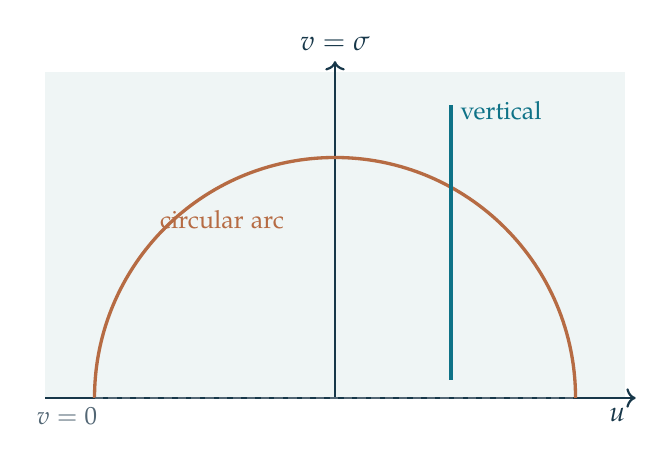
\begin{tikzpicture}[x=.92cm,y=.92cm]
 \fill[coursepale](-4,0)rectangle(4,4.5);
 \draw[->,courseink,thick](-4,0)--(4.15,0)node[below left]{\(u\)};
 \draw[->,courseink,thick](0,0)--(0,4.65)node[above]{\(v=\sigma\)};
 \draw[coursecopper,very thick](-3.32,0) arc[start angle=180,end angle=0,radius=3.32];
 \draw[courseteal,very thick] (1.6,.25)--(1.6,4.05);
 \draw[coursemuted,densely dashed](-3.32,0)--(3.32,0);
 \node[courseteal,above right,font=\small]at(1.6,3.7){vertical};
 \node[coursecopper,above right,font=\small]at(-2.55,2.2){circular arc};
 \node[coursemuted,below left,font=\small]at(-3.15,0){\(v=0\)};
\end{tikzpicture}
\end{center}
\end{frame}

\begin{frame}{Why a curved route can win}
At height \(v\), a small horizontal step \(du\) costs
\[
ds_F=\sqrt2\frac{|du|}{v}.
\]
\vspace{.51cm}
A path can trade some vertical travel for cheaper horizontal travel
by passing through larger standard deviations.
\vspace{.39cm}
The semicircular geodesic balances these contributions.
\end{frame}

\begin{frame}{Vertical geodesics and scale changes}
For two Gaussians with the same mean, the shortest route
is vertical in the half-plane.
\vspace{.37cm}
Its length is
\[
\highlightmath{d_F\big((\mu,\sigma_1),(\mu,\sigma_2)\big)
=\sqrt2\left|\ln\frac{\sigma_2}{\sigma_1}\right|}.
\]
\end{frame}

\coursepair{Distance between two centered Gaussians}{
Find the Fisher distance between
\[
N(0,1)\qquad\text{and}\qquad N(0,4).
\]
\vspace{.38cm}
Use the standard deviations in
\[
d_F=\sqrt2\left|\ln(\sigma_2/\sigma_1)\right|.
\]
}{
The two standard deviations are \(\sigma_1=1\) and \(\sigma_2=2\).
\vspace{.32cm}
Therefore
\[
\highlightmath{d_F=\sqrt2\ln2\approx.9803}.
\]
\vspace{.32cm}
Doubling standard deviation requires the same Fisher length,
regardless of the starting scale.
}

\begin{frame}{Constant Fisher speed on a vertical route}
A suitable time parameter is
\[
\highlightmath{v(t)=v_1\exp\left(t\ln\frac{v_2}{v_1}\right)},
\qquad 0\leq t\leq1.
\]
\vspace{.48cm}
Indeed \(v'(t)/v(t)=\ln(v_2/v_1)\), so
\[
\sqrt2\frac{|v'(t)|}{v(t)}
=\sqrt2\left|\ln\frac{v_2}{v_1}\right|.
\]
\end{frame}

\coursepair{A constant-speed scale midpoint}{
Let \(\sigma(0)=1\), \(\sigma(1)=4\), with fixed mean.
\vspace{.51cm}
Find the midpoint \(\sigma(1/2)\) along the
constant-Fisher-speed geodesic.
\vspace{.32cm}
How does it compare with the arithmetic midpoint \(2.5\)?
}{
With \(\sigma(t)=\exp(t\ln4)=4^t\),
\[
\highlightmath{\sigma(1/2)=\sqrt4=2}.
\]
\vspace{.44cm}
The Fisher midpoint in scale is the geometric mean
\(\sqrt{\sigma_1\sigma_2}\), rather than the arithmetic mean.
}

\begin{frame}{A formula for any pair of Gaussians}
Write \(P_i=(\mu_i,\sigma_i)\), with \(\sigma_i>0\).
Their Fisher distance is
\[
\highlightmath{d_F(P_1,P_2)=\sqrt2\,\operatorname{arcosh}\left(
1+\frac{(\mu_1-\mu_2)^2+2(\sigma_1-\sigma_2)^2}
{4\sigma_1\sigma_2}\right)}.
\]
\vspace{.43cm}
The expression inside \(\operatorname{arcosh}\) is at least one.
\end{frame}

\coursepair{Equal-width Gaussians, separated means}{
Take two distributions with
\[
(\mu_1,\sigma_1)=(-\sqrt2,1),
\quad(\mu_2,\sigma_2)=(\sqrt2,1).
\]
\vspace{.35cm}
Evaluate the general Gaussian Fisher distance formula.
}{
Here \((\mu_1-\mu_2)^2=8\) and \(\sigma_1=\sigma_2=1\).
\vspace{.38cm}
The \(\operatorname{arcosh}\) argument is \(1+8/4=3\), so
\[
\highlightmath{d_F=\sqrt2\,\operatorname{arcosh}(3)
\approx2.493}.
\]
}

\begin{frame}{The geodesic between those two laws}
With \(u=\mu/\sqrt2\), the endpoints are
\((-1,1)\) and \((1,1)\).
\vspace{.35cm}
The geodesic lies on the semicircle
\[
\highlightmath{u^2+v^2=2,\qquad v>0}.
\]
\vspace{.40cm}
At its highest point, \(v=\sqrt2\); the geodesic
temporarily uses a wider Gaussian than either endpoint.
\end{frame}

\begin{frame}{Relative entropy between two Gaussians}
For \(P=N(\mu_1,\sigma_1^2)\) and
\(Q=N(\mu_2,\sigma_2^2)\),
\[
\highlightmath{D(P\Vert Q)=\ln\frac{\sigma_2}{\sigma_1}
+\frac{\sigma_1^2+(\mu_1-\mu_2)^2}{2\sigma_2^2}
-\frac12}.
\]
\vspace{.48cm}
Unlike the Fisher distance, KL divergence can change
when the two distributions are interchanged.
\end{frame}

\coursepair{Compare both KL directions}{
Let \(P=N(0,1)\) and \(Q=N(0,4)\).
\vspace{.41cm}
Using the Gaussian KL formula, find
\[
D(P\Vert Q)\quad\text{and}\quad D(Q\Vert P).
\]
\vspace{.25cm}
Which is larger?
}{
For \(P=N(0,1)\) and \(Q=N(0,4)\),
\[
\highlightmath{D(P\Vert Q)=\ln2-\frac38\approx.318},
\]
\[
\highlightmath{D(Q\Vert P)=\frac32-\ln2\approx.807}.
\]
\vspace{.18cm}
The wider law is further from the narrow one in this KL direction.
}

\begin{frame}{Two different kinds of boundary}
In the Gaussian family, the limit \(\sigma\to0\) is at
infinite Fisher distance: \(\sqrt2|\ln\sigma|\to\infty\).
\vspace{.48cm}
In a finite categorical family, a probability coordinate can
approach zero in finite Fisher distance.
\vspace{.44cm}
Both spaces carry Fisher metrics, yet their global geometries differ.
\end{frame}

\begin{frame}{A geometric map of the course}
\begin{enumerate}
\setlength{\itemsep}{.38cm}
\item Replicator equations describe motion of distributions.
\item Entropy and KL divergence measure information and discrepancy.
\item The Fisher metric measures changes in probability laws.
\item Natural gradients and geodesics use that metric to describe motion and distance.
\end{enumerate}
\end{frame}

\begin{frame}{One last comparison}
The categorical Fisher manifold is a spherical orthant;
the Gaussian location-scale family is a hyperbolic half-plane.
\vspace{.48cm}
On both spaces, a point represents a distribution,
a tangent vector represents its change,
and a metric measures that change.
\vspace{.48cm}
That common structure is the geometry of information.
\end{frame}
\end{document}
